%version of 12-14-18

\chapter{GRAPH-THEORETIC CONCEPTS AND ENTITIES}
\label{Ch:Graphs-Trees}
\index{Graphs}

Graphs provide one of the richest technical and conceptual frameworks
in the world of computing.  They provide concrete representations of
manifold data structures, hence must be well understood in preparation
for a ``Data Structures and Algorithms'' course.  They embody tangible
abstractions of relationships of all sorts, hence must be well
understood in order to discuss entities as varied as web-search
engines and social networks with precision and rigor.  As with most of
the topics we discuss in this text, graph-oriented concepts must be
taught ``in layers''.  All students should be conversant with the use
of graphs to represent and reason about a vast array of complicated
relationships---ranging from taxonomies (including intra-family
structures) to link-based data structures to interconnectivity within
social media, and on and on---but the degree of sophistication that an
individual student requires depends both on the abilities of the
student and the range of graph-modeled concepts that will appear in
the student's program.  The most-basic concepts in this chapter should
be understood by all students in any academic program that includes a
computation-oriented component---although each concept can be
developed with more texture and nuance within the context of specific
application domains; the more advanced concepts should be selected
with care, based on the instructor's perception of students' needs, in
the light of the ever-growing importance of concepts involving
interconnectivity.

Many developments in computing technology over recent decades have
made it imperative that graphs no longer be viewed by students as the
static objects introduced early in the history of computational
studies.  For instance, while it was innovative in the 1960s to employ
graphs computationally as abstractions of data structures, such a view
is standard today.  Similar remarks, perhaps with differing dates, can
be made about graphs as vehicles for representing the flow of control
and information and as vehicles for representing interconnectivity
among both concepts and populations.  Applications ranging from
databases to web-search engines to social networks demand an
appreciation of graphs as dynamic objects.  This change in perspective
affects many aspects of the mathematical prerequisites for any
academic program that includes a computation-oriented component.


\section{An Intoduction to Graphs}
\label{sec:Graph-general}

\subsection{An informal overview}
\label{sec:graphs-informal}

The basic components of a graph $\g$ are its {\em nodes/vertices}
\index{Graphs!nodes} \index{Graphs!vertices} \index{node (of a graph)}
\index{vertex (of a graph)} (one encounters both terms in the
literature) and its {\em edges} \index{Graphs!edges} \index{edge (of a
  graph)} that interconnect them.  (The singular form of ``vertices''
is {\it vertex}.)  \index{Graphs!vertex} \index{vertex (of a graph)}
When graph $\g$ is {\em undirected}, \index{Graphs!undirected} each of
its edges connotes some sort of sibling-like relationship among nodes
of ``equal'' status.  When graph $\g$ is {\em directed}
\index{Graphs!directed} (sometimes referred to as a {\em digraph}),
\index{digraph} \index{Graphs!digraphs} each of its edges connotes an
``unequal'' relationship such as parenthood or priority or dependence;
edges in directed graphs are often termed {\em
  arcs}. \index{Graphs!arc} \index{arc (of a directed graph)}
\index{arc (of a digraph)} In many situations involving directed
graphs, it is important to recognize the {\em dual}
\index{Graphs!digraph!dual} of a digraph $\g$.  This dual---which is
usually denoted by some notational embellishment of ``$\g$'', such as
$\widehat{\g}$---is the digraph obtained by {\em reversing} all of
$\g$'s arcs.  One sometimes encounters situations when arguments
about, or operations on, a digraph $\g$ can be ``translated'' to
arguments about, or operations on, $\widehat{\g}$ with only clerical
effort.  A {\em subgraph} $\g'$ of a graph $\g$ is a graph whose nodes
are a subset of $\g$'s and whose edges are a subset of $\g$'s that
interconnect only nodes of $\g'$.  A {\em path} \index{Graphs!path}
\index{path (in a graph)} in an undirected graph is a sequence of
nodes within which every adjacent pair is connected by an edge.  A
path is a {\em cycle} \index{Graphs!cycle} \index{cycle (in a graph)}
if all nodes in the sequence are distinct, except for the first and
last, which are identical.  Paths and cycles in directed graphs are
defined similarly, except that every adjacent pair of nodes must be
connected by an arc, and all arcs must ``point in the same
direction.''

The special class of graphs called {\it trees} \index{Graphs!trees}
\index{Trees} occupy a place of honor within both the mathematical
field called {\it graph theory} and the vernacular.  Mathematically
speaking, a tree $\t$ is a graph that contains no cycles: $\t$ is thus
the embodiment of ``pure'' connectivity.  As one would expect from the
vernacular, a set of trees is called a {\it forest}. \index{forest (of
  trees)} Just as with graphs, there is a directed version of trees.
Within a directed tree $\t$, one singles out two special classes of
nodes: A {\it root (node)} \index{Trees!root (node)} \index{root (of a
  directed tree)} of $\t$ has no entering arcs; a {\it leaf (node)}
\index{Trees!leaf (node)} \index{leaf (of a directed tree)} of $\t$
has no exiting arcs.  The reader is certainly familiar with the use of
rooted directed trees to represent family trees and corporate
hierarchies.

\subsection{Generic Graphs: Directed and Undirected}
\label{sec:digraphs}

A {\it directed graph} \index{Graphs!directed} ({\it digraph},
\index{digraph} for short) $\g$ is given by a set of {\it nodes}
\index{Graphs!node}
\index{$\n_{\fg}$: set of nodes of graph $\g$}
$\n_{\fg}$ and a set of {\it arcs}
\index{Graphs!digraph!arcs}
(or {\it directed edges}) $\a_{\fg}$.
\index{$\a_{\fg}$: set of arcs of digraph $\g$}
Each arc of $\g$ has the form $(u \rightarrow v)$,
\index{$\rightarrow$: arc in a directed graph}
where $u, v \in \n_{\fg}$; we say that this arc goes {\em from} $u$
{\em to} $v$.  A {\it path} 
\index{Graphs!path in a digraph}
\index{path in a digraph}
in the digraph $\g$ is a sequence of arcs that share adjacent
endpoints, as in the following $(n-1)$-arc path from node $u_1$ to
node $u_n$ in $\g$:
\begin{equation}
\label{eq:di-path}
(u_1 \rightarrow u_2), \ (u_2 \rightarrow u_3), \ \ldots, \ (u_{n-2}
        \rightarrow u_{n-1}), \ (u_{n-1} \rightarrow u_n).
\end{equation}
The path described in (\ref{eq:di-path}) makes sense only when every
node $u_i$ belongs to $\n_{\fg}$ and every arc $(u_i \rightarrow u_j)$
belongs to $\a_{\fg}$.  The {\it length} of path (\ref{eq:di-path}) is
the number of arcs---i.e., $n-1$; and the existence of the path means
that the {\it distance} \index{distance in a digraph}
\index{digraph!distance} \index{Graphs!distance in a digraph} from
$u_1$ to $u_n$ in $\g$ is no greater than $n-1$.   (There may exist
shorter paths in $\g$ from $u_1$ to $u_n$.)

\medskip

It is sometimes useful to endow the arcs of a digraph with labels from
an alphabet $\Sigma$.  When so endowed, the path (\ref{eq:di-path})
would be written
\[
(u_1 \stackrel{\lambda_1}{\rightarrow} u_2), \ 
(u_2 \stackrel{\lambda_2}{\rightarrow} u_3), \ \ldots, \ 
(u_{n-2} \stackrel{\lambda_{n-2}}{\rightarrow} u_{n-1}), \ 
(u_{n-1} \stackrel{\lambda_{n-1}}{\rightarrow} u_n),
\]
where the $\lambda_i$ denote symbols from $\Sigma$.  If $u_1 = u_n$,
then we call the preceding path a {\em cycle}.\index{cycle (in a digraph)}

\medskip

An {\em undirected graph} $\h$ is given by a set of nodes $\n_{\fh}$
and a set $\e_{\fh}$ 
\index{$\e_{\fh}$: the set of edges of the undirected  graph $\h$}
of $2$-element subsets of $\n_{\fh}$.  Each of these subsets is called
an {\it edge (of $\h$)}.
\index{Graphs!edge} \index{edge (in a graph)}
One can, thus, view the undirected graph $\h$ as being obtained from a
directed graph $\bar{\h}$ by removing the directionality of
$\bar{\h}$'s arcs.  Whereas we say: \\
\hspace*{.35in}the {\em arc} $(u,v)$ goes {\em from} node $u$ {\em to}
node $v$ \\
we say: \\
\hspace*{.35in}the undirected edge $\{u,v\}$ goes {\em between} nodes
$u$ and $v$ \\
or, more simply: \\
\hspace*{.35in}the undirected edge $\{u,v\}$ {\em connects} nodes $u$
and $v$.  \\
One can view an undirected graph as asserting ``pure'' connectivity,
whereas directed graphs assert some form of priority or
directionality.

A {\it path} in an undirected graph \index{Graphs!path in undirected
  graph} \index{path in and undirectd graph} is a sequence of
edges---i.e., of $2$-element sets of nodes---such that adjacent edges
share a node.  For illustration, an $(n-1)$-edge path that connects
nodes $u$ and $v$ in the undirected graph $\h$ has the form
\begin{equation}
\label{eq:undi-path}
\{u, u_1\}, \ \{u_1, u_2\}, \ \{u_2, u_3\}, \ \ldots, \ \{u_{n-2},
u_{n-1}\}, \ \{u_{n-1}, v\}
\end{equation}
The path described in (\ref{eq:undi-path}) makes sense only when every
node $u_i$ belongs to $\n_{\fh}$ and every edge $(u_i \ u_j\}$ belongs
to $\e_{\fh}$.  The {\it length} of path (\ref{eq:undi-path}) is the
number of edges---which is $n-1$ in this example; and the existence of
the path means that the {\it distance} \index{distance in a graph}
\index{Graphs!distance} {\it between} $u$ and $v$ in $\h$ is no
greater than $n-1$.  (There may exist shorter paths that connect $u$
and $v$.)

\medskip

{\em Undirected} graphs are usually the default concept, in the
following sense: When $\g$ is described as a ``graph,'' with no
qualifier ``directed'' or ``undirected,'' it is usually understood
that $\g$ is an undirected graph.

\medskip

For each edge $\{u,v\} \in \e_{\fh}$, we call nodes $u$ and $v$ {\it
  neighbors} (in $\h$).
\index{neighbor node!in a graph}
The {\it degree}
\index{degree of a node in an undirected graph}
of a node $u \in \n_{\fh}$ is the number of neighbors that $u$ has.

We sometimes use the term {\it neighbor} within the context of {\em
  directed} graphs also.  If we say that nodes $u$ and $v$ are
neighbors in the directed graph $\g$,
\index{neighbor node!in a directed graph}
then we mean that $\a_{\fg}$ contains at least one of the arcs $(u
  \rightarrow v)$ or $(v \rightarrow u)$.  More typically, we use
  terminology that is more faithful to digraph $\g$'s directedness.
If $\a_{\fg}$ contains the arc $(u \rightarrow v)$, then we would call
  $v$ a {\it (direct) successor} of $u$
\index{digraph!successor node}
\index{successor node in a directed graph}
and we would call $u$ a {\it (direct) predecessor} of $v$
\index{digraph!predecessor node}
\index{predecessor node in a directed graph}
The term {\it parent} often replaces ``predecessor node'', and the
term {\it child} often replaces ``successor node'', especially when
$\g$ is a directed {\em tree}.  Acknowledging the distinction between
predecessors and successors in digraphs, we usually split the notion
of the degree of a node within a digraph into the {\it indegree} and
the {\it outdegree} of node $u$:
\begin{itemize}
\item
The {\it indegree} of node $u \in \n_{\fg}$
\index{digraph!indegree}
is the number of nodes $v \in \n_{\fg}$ such that $(u \rightarrow v)$
is an arc of $\g$.
\item
Symmetrically, the {\it outdegree} of node $u \in \n_{\fg}$
\index{digraph!outdegree}
is the number of nodes $v \in \n_{\fg}$ such that $(v \rightarrow u)$
is an arc of $\g$.
\end{itemize}

\noindent {\it Distance and diameter in a digraph.}
\index{digraph!distance between two nodes}
Extrapolating from our discussion of path (\ref{eq:di-path}): The {\it
  distance} from node $u_1$ to node $u_n$ in the digraph $\g$ is the
smallest number of arcs in any path from $u_1$ to $u_n$.  In detail:
\begin{equation}
\label{eq:di-distance-defn}
 \mbox{\sc distance}(u_1, u_n) \ \ \left\{
\begin{array}{cll}
= & 0 & \mbox{  if  } \ u_1 = u_n \\
\leq & n-1 & \mbox{  if there is a path } \ (\ref{eq:di-path})
\ \mbox{ from $u_1$ to $u_n$} \\
= & \infty & \mbox{  if there is no path } \ (\ref{eq:di-path})
\ \mbox{ from $u_1$ to $u_n$}
\end{array}
\right.
\end{equation}
The {\it diameter} \index{diameter in a digraph}
\index{digraph!diameter} of a directed graph $\g$ is the largest
distance between two nodes of $\g$, i.e., the largest number $d$ for
which there exist nodes $u_1, u_n \in \n_{\fg}$ such that {\sc
  distance}$(u_1, u_n) = d$.  Note that when discussing digraphs, we
always use {\em directed} paths when defining distance.

\medskip

\noindent {\it Distance and diameter in an undirected graph.}
\index{Graphs!!distance between two nodes}
\index{diameter in a graph}
Extrapolating from our discussion of path (\ref{eq:undi-path}): The
{\it distance between} node $u_1$ and node $u_n$ in the graph $\g$ is
the smallest number of edges in any path from $u_1$ to $u_n$.  In
detail:
\begin{equation}
\label{eq:distance-defn}
 \mbox{\sc distance}(u, v) \ \ \left\{
\begin{array}{cll}
= & 0 & \mbox{  if  } \ u = v \\
\leq & n-1 & \mbox{  if there is a path } \ (\ref{eq:di-path})
\ \mbox{ between $u$ and $v$} \\
= & \infty & \mbox{  if there is no path } \ (\ref{eq:di-path})
\ \mbox{ between $u$ and $v$}
\end{array}
\right.
\end{equation}
The {\it diameter} \index{diameter in a graph} \index{Graphs!diameter}
of an undirected graph $\h$ is the largest distance between two nodes
of $\h$, i.e., the largest number $d$ for which the exist nodes $u_1,
u_n \in \n_{\fh}$ such that {\sc distance}$(u_1, u_n) = d$.  Note that
when discussing undirected graphs, we always use {\em undirected}
paths when defining distance.


\subsection{Trees}
\label{sec:Trees}

The special class of graphs called {\it trees} \index{Graphs!trees}
\index{Trees} occupy a place of honor within both the mathematical
field called {\it graph theory} and within the vernacular.

Mathematically speaking, a tree is a graph that contains no cycles.  A
tree is thus the embodiment of ``pure'' connectivity: it provides the
minimal interconnection structure that provides paths that connect
every pair of nodes.  As one might expect from the vernacular, a set
of trees is called a {\it forest}. \index{forest (of trees)}

Just as with graphs, there is a {\em directed} version of trees, which
is formed by replacing the (unoriented) edges of an undirected tree by
(oriented) arcs.  Within a directed tree, one often says that an arc
goes from a {\it parent node} \index{Trees!parent node} to a {\it
  child node} \index{Trees!child node}.  Extending this
anthropomorphic metaphor, one often talks about the {\it ancestor(s)}
\index{Trees!ancestor node} and {\it descendant(s)}
\index{Trees!descendant node} of a tree-node.  We single out two
special classes of nodes of a directed tree: A {\it root (node)}
\index{Trees!root (node)} \index{root (of a directed tree)} is defined
by its having no entering arcs; a {\it leaf (node)} \index{Trees!leaf
  (node)} \index{leaf (of a directed tree)} is defined by its having
no exiting arcs.

\[ \approx \approx \approx \approx \approx \approx \approx \approx \approx \approx \]
Sociologically, the historical {\it atomic family tree} \index{family
  tree} has two roots, representing the matriarch and patriarch of the
family.  The entirety of the tree represents a single family
generationally, before any children form their own families.  All
child-nodes in this genre of tree are the roots of singly-rooted
subtrees of the entire family tree.  The leaves of the tree are the
childless descendants of the roots.  Note that, while we are using
anthropomorphic language here, we could be discussing other genres of
``family'', as, e.g., many types of biological taxonomies.
\[ \approx \approx \approx \approx \approx \approx \approx \approx \approx \approx \]

Among rooted directed trees, an important subclass comprises those
that have a {\em single root} which has a directed path to every other
node.  The length of each such directed path is often used to label
the {\it generation}
\index{generation of a node in a singly-rooted directed tree}
of the node at the end of the path: root, child, grandchild,
great-grandchild, etc.
Every node of the tree is the root of a singly-rooted directed
subtree of the entire tree.  All subtrees that are rooted at nodes of
the same generation are mutually disjoint.

\[ \approx \approx \approx \approx \approx \approx \approx \approx \approx \approx \]
A singly-rooted tree represents a {\it hierarchy}.
\index{Trees!singly-rooted!hierarchy} \index{hierarchy} Given two
directed subtrees within a hierarchy, either the root of one of the
subtrees is a descendant of the root of the other, or the two subtrees
are are mutually disjoint.
\[ \approx \approx \approx \approx \approx \approx \approx \approx \approx \approx \]

More formally: {\em rooted trees} are a class of {\em acyclic}
digraphs.  Paths in trees which start at the root are often called
{\em branches}.  The {\em acyclicity} of a tree $\t$ means that for
any branch of $\t$ of the form (\ref{eq:di-path}), we cannot have $u_1 =
u_n$, for this would create a cycle.  Each singly-rooted tree $\t$ has
a designated {\em root node} \index{Trees!root node} $u_n \in
\n_{\ft}$ that resides at the end of a branch (\ref{eq:di-path}) that
starts at $r_{\ft}$ (so $u_1 = r_{\ft}$) is said to reside at {\em
  depth} $n-1$ in $\t$; by convention, $r_{\ft}$ is said to reside at
depth $0$.  \index{depth of a node in a singly-rooted trees} $\t$'s
root $r_{\ft}$ has some number (possibly $0$) of arcs that go from
$r_{\ft}$ to its {\em children,} each of which thus resides at depth
$1$ in $\t$; in turn, each child has some number of arcs (possibly
$0$) to its children, and so on.  For each arc $(u \rightarrow v) \in
A_{\ft}$, we call $u$ a {\it parent} \index{Trees!parent node} of $v$,
and $v$ a {\it child} \index{Trees!child node} of $u$, in $\t$;
clearly, the depth of each child is one greater than the depth of its
parent.  Every node of $\t$ except for $r_{\ft}$ has precisely one
parent; $r_{\ft}$ has no parents.  A childless node of a tree is a
{\em leaf}.  \index{Trees!leaf node} The transitive extensions of the
parent and child relations are, respectively, the {\em ancestor}
\index{Trees!ancestor node} and {\em descendant}
\index{Trees!descendant node} relations.  The {\em degree}
\index{degree (of a node in a tree)} of a node $v$ in a tree is the
number of children that the node has, call it $c_v$.  If every nonleaf
node in a tree has the same degree $c$, then we call $c$ the {\em
  degree of the tree}.
\index{degree of a tree}

It is sometimes useful to have a symbolic notation for the ancestor
and descendant relations.  To this end, we write $(u \Rightarrow v)$
\index{$\Rightarrow$: ancestor/descendant in a rooted tree} to
indicate that node $u$ is an {\it ancestor} of node $v$, or
equivalently, that node $v$ is a {\it descendant} of node $u$.  If we
decide that we are not interested in {\em really distant} descendants
of the root of a tree $\t$, then we can {\em truncate} \index{truncated}
$\t$ at a desired depth $d$ by removing all nodes whose depths exceed
$d$.  We thereby obtain the {\em depth-$d$ prefix} of $\t$.

\ignore{****************
Figure \ref{fig.graph-samples} depicts an arc-labeled rooted tree $\t$
whose arc labels come from the alphabet $\{a,b\}$.  $\t$'s arc-induced
relationships are listed in Table~\ref{tab.graph-samples}.
\begin{figure}[htb]
\centerline{\epsfig{figure=graph.sample.eps,height=4truecm}}
\caption{An arc-labeled rooted tree $\t$ whose arc labels come from
  the alphabet $\{a,b\}$.  (Arc labels have no meaning; they are just
  for illustration.)
\label{fig.graph-samples}}
\end{figure}
\begin{table}[htb]
{\small
\begin{center}
\fbox{
\begin{tabular}{c||c|c|c|c}
\multicolumn{5}{c}{The arc-labeled rooted tree $\t$ of
  Figure \ref{fig.graph-samples}} \\
\hline
Node            & Children & Parent & Descendants & Ancestors \\
\hline
\hline
$r_{\ft} = u_0$ 
& $u_1$
& none & 
$u_1, u_2, \ldots, u_k, v_1, v_2, \ldots, v_k,
w_1, w_2, \ldots, w_k$
& none \\
\hline
$u_1$
& $u_2, v_1$
& $u_0$ & 
$u_2, \ldots, u_k, v_1, v_2, \ldots, v_k, w_1, w_2, \ldots, w_k$
& $u_0$ \\
\hline
$u_2$
& $u_3, v_2$
& $u_1$ & 
$u_3, \ldots, u_k, v_2, \ldots, v_k, w_2, \ldots, w_k$
& $u_0$ \\
\hline
 $\vdots$ & $\vdots$ & $\vdots$ &  $\vdots$ &  $\vdots$ \\
\hline
$u_k$
& $v_k$ 
& $u_{k-1}$ & 
$v_k, w_k$
& $u_0, u_1, \ldots, u_{k-1}$ \\
\hline
$v_1$
& $w_1$ 
& $u_1$ & 
$w_1$
& $u_0, u_1$ \\
\hline
$v_2$
& $w_2$
& $u_2$ & 
$w_2$
& $u_0, u_1, u_2$ \\
\hline
 $\vdots$ & $\vdots$ & $\vdots$ &  $\vdots$ &  $\vdots$ \\
\hline
$v_k$
& $w_k$
& $u_k$ & 
$w_k$
& $u_0, u_1, \ldots, u_k$ \\
\hline
$w_1$
& none
& $v_1$ & 
none
& $u_0, u_1, v_1$ \\
\hline
$w_2$
& none &
$v_2$ & 
none
& $u_0, u_1, u_2, v_2$ \\
\hline
$w_k$
& none
& $v_k$ & 
none
& $u_0, u_1, \ldots, u_k, v_k$
\end{tabular}
}
\end{center}
}
\caption{A tabular description of the rooted tree $\t$ of
  Figure \ref{fig.graph-samples}.  \label{tab.graph-samples}}
\end{table}
*********************}

\subsection{Other Important Families of Graphs}
\label{sec:graphs-important-families}

The mathematical discipline called graph theory is an important source
of formal aids for the activities of designing, analyzing, utilizing,
and verifying computer systems.  Of course, computer systems are
designed by humans.  Among other consequences of this fact is the
observations that the graphs that are among the most commonly used to
structure systems tend to be rather uniform in structure, in a variety
of possible ways.  Such graphs, when drawn, often exhibit a lot of
structural symmetry.  One popular form of symmetry is {\it degree
  regularity}: an undirected graph $\g$ is {\it regular}
\index{Graphs!regular} if all nodes of $\g$ have the same degree.  Not
surprisingly, there is a directed version of regular embodied in the
symmetric notions of {\it in-regularity}
\index{Graphs!directed!in-regular} and {\it out-regularity}.
\index{Graphs!directed!out-regular}

We now describe five families of regular graphs that have proven
useful over the history of digital computing, and we expose some basic
properties of each, including its diameter.  Each of these graphs is
available in both a directed and an undirected version.

*** DESCRIBE MOTIVATION / CHOICE OF GRAPHS***

Say Especially when the graphs are studied within the context of {\em
  hardware}---i.e, as the network that underlies a parallel
architecture by interconnecting its processors

Throughout, the parameters that describe our graph families range over
the positive integers; i.e., each occurrence of $n$ below ranges over
$\N^+$.

\subsubsection{The cycle-graph}
\label{sec:cycle-graph}

For each positive integer $n \in \N^+$, both the {\it undirected
  order-$n$ cycle-graph} $\cc_n$ and the {\it directed order-$n$
  cycle-graph} $\widehat{\cc}_n$ \index{cycle graph} \index{cycle
  network} have {\it node-set}
\[ \n_{{\cal C}_n} \ = \ \n_{\widehat{{\cal C}}_n}
\ = \ \{ 0, \ 1, \ \ldots, \ n-1\}. \]
\begin{itemize}
\item
$\cc_n$ has $n$ edges; its {\it edge-set} is
\[ \e_{{\cal C}_n} \ = \
\big\{ \{i, \ i+1 \bmod n\} \ \ | \ \ i \in \{0, \ 1, \ \ldots,
\ n-1\} \big\}.
\]
  \begin{itemize}
  \item \index{cycle graph!node-degree}
$\cc_n$ is a regular network: each node has degree $2$.

Specifically, each node $i$ of $\cc_n$ has its {\it predecessor} $i-1
\bmod n$ \index{cycle graph!predecessor node} \index{cycle
  graph!successor node} and its {\it successor} $i+1 \bmod n$ .
  \item \index{cycle graph!diameter}
$\cc_n$ has diameter $\lfloor n/2 \rfloor$.

Direct calculation shows that $\cc_n$'s diameter is no larger than
this.  The fact that this is, in fact, the graphs's diameter is
witnessed by the distance betewen each node $k \in \n_{{\cal C}_n}$
and its antipodal node $k + \lfloor n/2 \rfloor \bmod n$.
  \end{itemize}

\item
$\widehat{\cc}_n$ has {\it arc-set}
\[ \a_{\widehat{{\cal C}}_n} \ = \ 
\big\{ (i \rightarrow i+1 \bmod n) \ \ | \ \ i \in \{0, \ 1, \ \ldots, \ n-1\} \big\}
\]
  \begin{itemize}
  \item \index{cycle graph!directed node-degree}
$\widehat{\cc}_n$ is a regular network: each node has the same
    indegree and the same outdegree.  Coincidentally both the common
    indegree and the common outdegree are $2$.
  \item
$\widehat{\cc}_n$ has (directed) diameter $n-1$.

Of course, $n-1$ is an upper bound on the diameter of any $n$-node
digraph.  The fact that this is, in fact, the graph's diameter is witnessed by
the directed distance from each node $k$ of $\widehat {\cc}_n$ 
to its predecessor node $k-1 \bmod n$. 
  \end{itemize}
\end{itemize}

\subsubsection{The {\em complete} graph}
\label{sec:complete-graph}
\index{complete graph}

For each positive integer $n \in \N^+$, both the {\it undirected
  order-$n$ complete-graph} $\k_n$ and the {\it directed order-$n$
  complete-graph} $\widehat{\k}_n$ \index{complete graph} have {\it
  node-set}
\[ \n_{{\cal K}_n} \ = \ \n_{\widehat{{\cal K}}_n}
\ = \ \{ 0, \ 1, \ \ldots, \ n-1\}. \]
\begin{itemize}
\item
$\k_n$ has $\displaystyle {n \choose 2}$ edges; its {\it edge-set} is
\[ \e_{{\cal K}_n} \ = \
\big\{ \{i, \ j\} \ \ | \ \ i,j \in \{0, \ 1, \ \ldots, \ n-1\}, \ i
\neq j \big\}.
\]
  \begin{itemize}
  \item \index{complete graph!node-degree}
$\k_n$ is a regular network: each node has degree $n-1$.

Every node $i$ of $\k_n$ is connected with all other nodes.

   \item \index{complete graph!diameter}
$\k_n$ has diameter $1$.

$\k_n$'s diameter is a direct consequence of its node-degrees, and vice versa.
  \end{itemize}

\item
$\widehat{\k}_n$ has $(n-1)n$ arcs; its {\it arc-set} is
\[ \a_{\widehat{{\cal K}}_n} \ = \ 
\big\{ (i \rightarrow j) \ \ | \ \ i,j \in \{0, \ 1, \ \ldots, \ n-1\}
\big\}, \ i \neq j
\]
  \begin{itemize}
  \item
$\widehat{\k}_n$ is a regular network: each node has the same indegree
    and the same outdegree.  Both the common indegree and the common
    outdegree are $n-1$.
  \item
$\widehat{\k}_n$ has (directed) diameter $1$.

As in the undirected case, there is a causal relationship between
$\widehat{\k}_n$'s diameter and its (in- and out-) node-degrees.
  \end{itemize}
\end{itemize}

\bigskip

The families of graphs we discuss in the coming subsections are among
the most important graph families when discussing parallel and
distributed computing (PDC).  All of these families have been used
both to design computer architectures that support PDC and to craft
algorithms that exploit the potential efficiencies---in computation
and communication---that one can achieve using PDC.

\subsubsection{The mesh network and the torus network}
\label{sec:mesh-torus}
\index{mesh and torus networks}

For positive integers $m, n \in \N^+$, both the $m \times n$ {\it mesh
  (network)} $\m_{m,n}$ and the $m \times n$ {\it toroidal network}
(or, {\it torus}) $\widetilde{\m}_{m,n}$ have {\it node-set}
\begin{eqnarray*}
\n_{\fm_{m,n}} \ = \ \n_{\widetilde{\fm}_{m,n}}
  & = & 
\{1, \ 2, \ldots, \ m\} \ \times \ \{1, \ 2, \ldots, \ n\} \\
  & = & 
\big\{ \langle i, \ j \rangle \ \ | \ \ 
\big[ i \in \{1, \ 2, \ldots, \ m\} \big], \ \
\big[ j \in \{1, \ 2, \ldots, \ n\} \big]
\big\}
\end{eqnarray*}

\begin{itemize}
\item
$\m_{m,n}$ has $(m-1)n \ + \ (n-1)m$ edges; its {\it edge-set} is
\begin{eqnarray*}
\e_{\fm_{m,n}} & = & 
\big\{
\{ \{ i, j \}, \ \{ i+1, j \} \ \ | \ \
1 \leq i < m, \ \ 1 \leq j \leq n \} \\
  &  & \hspace*{.1in} \cup
\{ \{ i, j \}, \ \{ i, j+1 \} \ \ | \ \
1 \leq i \leq m, \ \ 1 \leq j < n \}
\big\}
\end{eqnarray*}

  \begin{itemize}
  \item
    \begin{itemize}
    \item
The subgraph of $\m_{m,n}$ defined by the node-set
\[ \{ \langle i, \ j \rangle  \ \ | \ \ \left[i \in \{1, 2, \ldots,
  m\}\right], \ \ \left[1 \leq j < n\right]\}
\]
and all edges both of whose endpoints belong to that set is called the
$i$th {\it row} of $\m_{m,n}$
\index{row of a mesh graph}
\index{mesh graph!row}
Dually, the subgraph of $\m_{m,n}$ defined by the node-set
\[ \{ \langle i, \ j \rangle  \ \ | \ \ \left[j \in \{1, 2, \ldots,
  n\}\right], \ \ \left[1 \leq i < m\right] \}
\]
and all edges both of whose endpoints belong to that set is called the
$j$th {\it column} of $\m_{m,n}$.
\index{column of a mesh graph}
\index{mesh graph!column}
     \item
Nodes $\langle 1, \ 1 \rangle$, $\langle 1, \ n \rangle$, $\langle m,
\ 1 \rangle$, and $\langle m, \ n \rangle$ are the {\it corner nodes}
(or, just {\it corners}) of $\m_{m,n}$.
\index{corner (node) of a mesh graph}
\index{mesh graph!corner (node)}
     \item
The path-graph consisting of the node-set
\[ \{ \langle 1, \ 1 \rangle, \ \langle 1, \ 2 \rangle, \ldots, \
\langle 1, \ n \rangle \}
\]
together with all edges of $\m_{m,n}$ both of whose endpoints belong
to this set, is the {\it top edge} of $\m_{m,n}$.
\index{top edge of a mesh graph}
\index{mesh graph!top edge}

The other edges of $\m_n$ are defined analogously:

\smallskip

The {\it bottom edge} of $\m_{m,n}$ is the path-graph built upon the
node-set
\[ \{ \langle m, \ 1 \rangle, \ \langle m, \ 2 \rangle, \ldots, \
\langle m, \ n \rangle \}
\]
\index{bottom edge of a mesh graph}
\index{mesh graph!bottom edge}

The {\it left edge} of $\m_{m,n}$ is the path-graph built upon the
node-set
\[ \{ \langle 1, \ 1 \rangle, \ \langle 2, \ 1 \rangle, \ldots, \
\langle m, \ 1 \rangle \}
\]
\index{left edge of a mesh graph}
\index{mesh graph!left edge}

The {\it right edge} of $\m_{m,n}$ is the path-graph built upon the
node-set
\[ \{ \langle 1, \ n \rangle, \ \langle 2, \ n \rangle, \ldots, \
\langle m, \ n \rangle \}
\]
\index{left edge of a mesh graph}
\index{mesh graph!right edge}
     \end{itemize}

  \item \index{mesh graph!node-degree}
$\m_{m,n}$ is {\em not} a regular graph.  Its corner nodes each has
    degree $2$; its non-corner edge nodes each has degree $3$; its
\index{internal node of a mesh graph}
\index{mesh graph!internal node}
{\em internal nodes}---which are all non-edge nodes---each has degree
$4$

  \item \index{mesh graph!undirected diameter}
The diameter of $\m_{m,n}$ is $m+n-2$, as witnessed by the distance
between nodes $\langle 1, \ 1 \rangle$ and $\langle 2, \ n \rangle$.
  \end{itemize}

\item
$\widetilde{\m}_{m,n}$ has $2mn$ arcs; its {\it arc-set} is
\begin{eqnarray*}
\a_{\widetilde{\m}_{m,n}} & = &
\big\{
\{ (\langle i, \ j \rangle \rightarrow \langle i+1 \bmod m, \ j
\rangle) \ \ | \ \ 1 \leq i \leq m, \ \ 1 \leq j \leq n \} \\
  &  & \hspace*{.1in} \cup
\{ (\langle i, \ j \rangle \rightarrow \langle i, \ j+1 \bmod n
\rangle) \ \ | \ \ 1 \leq i \leq m, \ \ 1 \leq j \leq n \}
\big \}
\end{eqnarray*}

  \begin{itemize}
  \item
The subgraph of $\widetilde{\m}_{m,n}$ defined by the node-set
\[ \{ \langle i, \ j \rangle  \ \ | \ \ \left[i \in \{1, 2, \ldots,
  m\}\right], \ \ \left[1 \leq j \leq n\right]\}
\]
and all edges both of whose endpoints belong to that set is called the
$i$th {\it row} of $\widetilde{\m}_{m,n}$
\index{torus graph!row}
Dually, the subgraph of$\widetilde{\m}_{m,n}$ defined by the node-set
\[ \{ \langle i, \ j \rangle  \ \ | \ \ \left[j \in \{1, 2, \ldots,
  n\}\right], \ \ \left[1 \leq i \leq m\right] \}
\]
and all edges both of whose endpoints belong to that set is called the
$j$th {\it column} of $\widetilde{\m}_{m,n}$.
\index{torus graph!column}
  \item
$\widetilde{\m}_{m,n}$ is a regular network; each node has degree $4$.
    Despite the fact that $\widetilde{\m}_{m,n}$ is an {\em
      undirected} graph, its arcs are commonly referred to via an
    anthropomorphic labeling, either as ``up, down, left, and right''
    or as ``north, south, west, and east''.
  \item \index{mesh graph!directed diameter}
$\widetilde{\m}_{m,n}$'s diameter is $\lfloor m/2 \rfloor \ + \
\lfloor n/2 \rfloor$.  This can be verified in analogy to the diameter
of the cycle-graph $\cc_n$.
  \end{itemize}
\end{itemize}


\subsubsection{The boolean hypercube}
\label{sec:hypercube}
\index{boolean hypercube}
\index{hypercube}

The graphs we focus on next have had a major impact on the world of
coding, especially in regard to codes that are {\em error correcting}
\cite{PetersonW81}, and the world of computing, especially in regard
to parallel and distributed computing
\cite{JohnssonH1989, SaadS89, Schwartz80}.  The cited sources give a
range of perspectives on the importance of {\it hypercube networks.}

\index{order-$n$ boolean hypercube}
The {\it order-$n$ boolean hypercube}, traditionally denoted $\q_n$,
is the $2^n$-node graph defined as follows.
\begin{itemize}
\item
{\it The recursive definition}. 
\index{order-$n$ boolean hypercube!recursive definition}
  \begin{itemize}
  \item
The order-$0$ boolean hypercube, $\q_0$, has a single node, and no
edges.
  \item
The order-$(k+1)$ boolean hypercube, $\q_{k+1}$, is obtained by taking
two copies of $\q_k$, call them $\q_k^{(1)}$ and $\q_k^{(2)}$, and
creating an edge that connects each node of $\q_k^{(1)}$ with the
corresponding node of $\q_k^{(2)}$.
  \end{itemize}
For illustration:
  \begin{itemize}
  \item
$\q_1$ consists of two nodes connected by a single edge.
  \item
$\q_2$ can be viewed as a ``square'', or equivalently, a copy of $\cc_4$.
  \item
$\q_3$ can be viewed as a ``cube'', i.e., as two copies of $\cc_4$
    with edges connecting corresponding nodes: Each of the following
    pairs of nodes are connected by an edge: the upper right
    corner-nodes, the upper left corner-nodes, the lower right
    corner-nodes, and the lower left corner-nodes.
  \end{itemize}

\item
{\it The direct definition}.
For each $n \in \N$, the nodes of the order-$n$ boolean hypercube,
$\q_n$, are all length-$n$ binary strings.  For illustration:
\index{order-$n$ boolean hypercube!direct definition}
\begin{eqnarray*}
\n_{{\fq}_0}
  & = & 
\{ \varepsilon \}, \ \ \mbox{ the length-$0$ {\em null string}} \\ 
\n_{{\fq}_1}
  & = &
\{ 0, \ 1 \} \\
\n_{{\fq}_2}
  & = & \{ 00, \ 01, \ 10, \ 11 \} \\
\n_{{\fq}_3}
  & = & \{ 000, \ 001, \ 010, \ 011, \ 100, \ 101, \ 110, \ 111 \} 
\end{eqnarray*}
Easily, for each value of $n$, $\q_n$ has $2^n$ nodes, for this is the
number of length-$n$ binary strings.

\medskip

For each value of $n$, each edge of $\q_n$ connects two node-strings
that differ in precisely one position.  This means that $\q_n$ has $n
2^{n-1}$ edges: To wit, each of its $2^n$ nodes has $n$ neighbors, so
the quantity $n 2^n$ counts each of $\q_n$'s edges twice---one for
each endpoint.  For illustration:
\begin{eqnarray*}
\a_{{\fq}_1}
  & = &
\big\{ \{ 0, \ 1 \} \big\} \\
\a_{{\fq}_2}
  & = & \big\{
\{ 00, \ 01 \}, \ \{ 00, \ 10\}, \
\{ 01, \ 11 \}, \ \{ 10, \ 11\} 
\big\} \\
\a_{{\fq}_3}
  & = & \big\{ 
\{000, \ 001\}, \
\{000, \ 010\}, \
\{000, \ 100\}, \
\{001, \ 011\}, \\
  &  & \hspace*{.2in}
\{001, \ 101\}, \
\{010, \ 011\}, \
\{010, \ 110\}, \
\{100, \ 101\}, \\
  &  & \hspace*{.2in}
\{100, \ 110\}, \
\{101, \ 111\}, \
\{011, \ 111\}, \
\{110, \ 111\}
\big\}
\end{eqnarray*}
\end{itemize}

\medskip

\noindent
It is easy to observe $\q_n$'s basic structural properties.
\begin{itemize}
\item \index{hypercube!node-degree}
$\q_n$ is a regular network: each of its $2^n$ nodes has degree $n$.

This follows from the fact that each arc of $\q_n$ rewrites a single
bit-position in the length-$n$ binary string that is the arc's source
node.

\item \index{hypercube!diameter}
$\q_n$ has diameter $n \ = \ \ln(|\n_{\fq_n}|)$.\footnote{Recall that
  $\ln n = \log_2 n$; see Section~\ref{sec:logarithmic-fns}.}

We address this issue formally.
\end{itemize}

\begin{prop}
\label{thm:hypercube-diameter}
For all $n \in \N^+$, $\q_n$ has diameter $n \ = \ \ln(|\n_{\fq_n}|)$.
\end{prop}

\begin{proof}
We prove this diameter bound by construction.  Focus on two arbitrary
nodes of $\q_n$:
\[ x \ = \ \alpha_1 \alpha_2 \cdots \alpha_n \ \ \ \mbox{ and } \ \ \
y \ = \ \beta_1 \beta_2 \cdots \beta_n
\]
One of the several paths in $\q_n$ from $x$ to $y$ is described
schematically as the following left-to-right, bit-by-bit rewriting of
$x$ as $y$ using arcs of $\q_n$
\[
x \ = \ \alpha_1 \alpha_2 \cdots \alpha_n \ \rightarrow \
\beta_1 \alpha_2 \cdots \alpha_n \ \rightarrow \
\beta_1 \beta_2\cdots \alpha_n \ \rightarrow \cdots \rightarrow\ 
\beta_1 \beta_2 \cdots \beta_n \ = \ y
\]
Since each bit of each string is rewritten once, the bound follows.
\qed
\end{proof}

\medskip

The fact that $\q_n$'s diameter is {\em logarithmic} in its size makes
$\q_n$ an efficient network for many tasks related to parallel
computing and communication.

\subsubsection{The de Bruijn network}
\label{sec:de-bruijn}
\index{de Bruijn network}
\index{de Bruijn graph}

While the family of hypercube networks has few competitors in the
world of parallel and distributed computing, in terms of performance
and ease of designing algorithms, it does have one major shortcoming
regarding its realization in hardware.  The basic problem is that the
order-$n$ hypercube has large node-degrees, specifically logarithmic
in the size of the network.  This feature makes the hypercubes actual
performance much lower than its theoretical performance.
Specifically, the size of the hypercube grows exponentially with the
common degrees of the network's nodes---this is the ``inverse'' way
of talking about logarithmic node-degrees---while the space in which
we (and our computers) live grows only cubically with linear
distance.  The resulting disparity means that the wires in a large
hypercube must inevitably be very long---in contrast to the unit-size
of idealized network-edges.  Consequently, electrical signals within a
large hyeprcube must travel long distances, which means that the
physical computer is much slower than its idealized version.  (One
finds a more technical discussion of this phenomenon in
\cite{Ullman84}.)

The preceding shortcoming of hypercubes led researchers to seek a
family of networks whose node-degrees stay constant even as one
deploys successively larger instances of the network.  A candidate
such network was discovered within the domain of coding theorists (as,
coincidentally, was the hypercube).  

In the mid-20-century, Dutch mathematican Nicolaas Govert de Bruijn
\index{de Bruijn, Nicolaas Govert} discovered a way to generate
compact sequences that contain all possible strings of a prespecified
length.  Focussing on {\em binary} strings---although de Bruijn's
strategy works for any finite alphabet---de Bruijn could generate a
string of length $2^n +n-1$ that contains every length-$n$ binary
string as a substring.  Quite appropriately, such a string is called a
{\it de Bruijn sequence}. \index{de Bruijn sequence} It is not obvious
that de Bruijn sequences exist for every $n$, but we now plant the
seeds of a proof that they do.  We begin by illustrating two sample
sequences in (\ref{eqn:deBruijn-seq}).
\begin{equation}
\label{eqn:deBruijn-seq}
\begin{array}{|l||c|c|}
\hline
n & \mbox{\sc Length-$n$ binary strings}
    & \mbox{\sc Order-$n$ de Bruijn sequence} \\
\hline
\hline
1 &
00, \ 01, \ 10, \ 11  & 00110 \\
\hline
2 &
\begin{array}{l}
000, \ 001, \ 010, \ 011, \\
100, \ 101, \ 110, \ 111 
\end{array}
  & 0001110100 \\
\hline
\end{array}
\end{equation}
The table in (\ref{eqn:deBruijn-seq}) spawns many interesting
questions:
\begin{itemize}
\item
Do de Bruijn sequences exist for every $n$?
\item
If so, 
  \begin{itemize}
  \item
How does one compute them?
  \item
Can one always find a de Bruijn sequence of length $2^n +n-1$?
  \item
Can one find de Bruijn sequences of length $< 2^n +n-1$?
  \end{itemize}
 {\Arny (SOME GOOD EXERCISES HERE)}  
\end{itemize}
The answers to all of these questions---and the connection of de
Bruijn sequences to the current chapter---reside in the family of
directed graphs called either {\it de Bruijn graphs} or {\it de Bruijn
  networks}.  \index{de Bruijn graph} \index{de Bruijn network} (The
term used varies by intended application---mainly, coding theory and
[the interconnection networks of] parallel computer architectures.  We
use the names interchangeably.)

For every integer $n \in \N^+$, the {\it order-$n$ de Bruijn network}
is the {\em directed} graph $\d_n$ whose nodes comprise the set of
length-$n$ binary strings\footnote{While {\em binary} de Bruijn
  networks are the most frequently encountered ones, one can also find
  de Bruijn networks whose nodes comprise all length-$n$ strings over
  larger finite alphabets.  Such extended families also find
  applications in coding theory.}  The sets $\n_{\fd_2}$ and
$\n_{\fd_3}$ appear in (\ref{eqn:deBruijn-seq}).

$\d_n$ is a regular directed graph; its nodes all have in-degree $2$
and outdegree-$2$.  Each node of $\d_n$ is a binary string of
length $n \geq 1$; hence it can be written in the form $\beta x$,
where $\beta \in \{0, \ 1\}$ is a {\it bit} (short for {\it binary
  digit}) and $x$ is a length-$(n-1)$ binary string.

The $2^{n+1}$ arcs of $\d_n$ come in pairs specified as follows.  For
each $\beta \in \{0,1\}$ and for each length-$(n-1)$ binary string
$x$, $\d_n$ has the two arcs
\[ (\beta x \rightarrow x0) \ \ \ \mbox{ and } \ \ \ 
(\beta x \rightarrow x1)
\]
We enumerate $\a_{\fd_3}$ in (\ref{eqn:deBruijn-arcs}).
\begin{equation}
\label{eqn:deBruijn-arcs}
\begin{array}{|ccccc|}
\hline
\mbox{\sc Source node} & & \mbox{\sc Target node} & & \mbox{\sc Target node} \\
\hline \hline
{\displaystyle
\left.
\begin{array}{c}
000 \\
001 \\
010 \\
011 \\
100 \\
101 \\
110 \\
111
\end{array}
\right\}
} &
\mbox{\sc goes to} 
  &
{\displaystyle
\left\{
\begin{array}{c}
000 \\
010 \\
100 \\
110 \\
001 \\
011 \\
101 \\
111
\end{array}
\right.
}
  &
\mbox{\sc and to}
  &
{\displaystyle
\left\{
\begin{array}{c}
001 \\
011 \\
101 \\
111 \\
000 \\
010 \\
100 \\
110
\end{array} 
\right.
}
 \\
\hline
\end{array}
\end{equation}

For each $n \in \N^+$, $\d_n$ has diameter $n$.  To see why this is
true, note that following any one of $\d_n$'s arcs, say from node $x$
to node $y$, consists of ``rewriting'' the length-$n$ string $x$ as
the length-$n$ string $y$.  The diameter bound therefore follows by
showing that, for any two string-nodes of $\d_n$, say node $u$ and
node $v$, one can rewrite string $u$ as string $v$ by traversing a
sequence of arcs---i.e., a directed path---of length at most $n$.
Observe, for instance, that the path in $\d_3$ described schematically
as follows
\[ 000 \ \rightarrow \ 001 \ \rightarrow \ 011 \ \rightarrow \ 111 \]
leads node $000$ to node $111$, by rewriting string $000$ as string
$111$.  The diameter bound is now an immediate consequence of the
following result.

\begin{prop}
\label{thm:deBruijn-hamiltonian}
For all $n \in \N^+$, $\d_n$ contains a {\em directed hamiltonian
  cycle}, 
\index{directed hamiltonian cycle in a digraph}
i.e., a length-$2^n$ directed cycle of the form
\begin{equation}
\label{eq:deBruijn-cycle}
 x \ \rightarrow \ y_1 \ \rightarrow \ y_2 \ \rightarrow \cdots
\ \rightarrow \ y_{2^n-1} \ \rightarrow \ x
\end{equation}
that contains every node of $\d_n$ precisely once; i.e.:
\begin{itemize}
\item
$\{x, \ y_1, \ y_2, \ldots, \ y_{2^n-1}\} \ = \ \n_{\fd_n}$.
\item
All of the ``$y$-nodes'' that appear in cycle
(\ref{eq:deBruijn-cycle}) differ from $x$ and from each other.
\end{itemize}
\end{prop}

The simplest proof of this result has two steps, each of which
introduces a topic we have not yet developed.

\medskip

\noindent {\bf (1)}
%
For any directed graph $\g$, the {\it line digraph} \index{line graph}
\index{line digraph} of $\g$, denoted $\l(\g)$, is the following
directed graph.
\begin{itemize}
\item
The nodes of $\l(\g)$ are the arcs of $\g$:
\[ \n_{{\cal L}({\cal G})} \ = \ \a_{\fg} \]
\item
For each pair of arcs of $\g$ of the form
\[ \big[a_{x,y} = (x \ \rightarrow \ y) \big] \ \ \ \mbox{ and } \ \ \ 
\big[a_{y,z} = (y \ \rightarrow \ z) \big]
\]
i.e, arcs such that the endpoint of the first arc is the source of the
second arc, $\l(\g)$ contains an arc $(a_{x,y} \ \rightarrow
\ a_{y,z})$.
\end{itemize}
The relevance of this topic to this section is that the line graph of
every de Bruijn network $\d_n$ is the ``next bigger'' de Bruijn
network, $\d_{n+1}$.  Let us verify this claim.

\begin{prop}
\label{thm:deBruin-linegraph}
For all $n \in \N^+$,
$\d_{n+1}$ is the line digraph of $\d_n$: $\d_{n+1} \ = \ \l(\d_n)$.
\end{prop}

\begin{proof}
Each node of $\l(\d_n)$ is an arc of $\d_n$, hence has the form
\[ (\beta x \ \rightarrow \ x \gamma) \]
for $x$ a length-$(n-1)$ binary string and $\beta, \gamma \in
\{0,1\}$.  Let us associate node $\beta x \gamma$ of $\d_{n+1}$ with
this node of $\l(\d_n)$.

\smallskip

Note first that each arc of $\d_{n+1}$ has the form
\[ (\delta y \varepsilon \ \rightarrow \ y \varepsilon \varphi), \]
where $y$ is a length-$(n-2)$ binary string and $\delta, \varepsilon,
\varphi \in \{0,1\}$.  By our association of nodes of $\d_{n+1}$ with
arcs of $\d_n$, this arc of $\d_{n+1}$ does, indeed, correspond to two
successive arcs of $\d_n$.   The first of these successive arcs
{\em enters} node $y \varepsilon$ of $\d_n$; the second {\em leaves}
that node.

Note next that, given any two successive arcs of $\d_n$, say
\[
(\rho \sigma z \ \rightarrow \ \sigma z \tau) \ \ \ \mbox { and } \ \ \
(\sigma z \tau \ \rightarrow \  z \tau \xi)
\]
where $z$ is a length-$(n-2)$ binary string and $\rho, \sigma, \tau,
\xi \in \{0,1\}$, there is, indeed, an arc of $\d_{n+1}$ of the form
\[ (\rho \sigma z \tau \ \rightarrow \ \sigma z \tau \xi) \]
This means that the digraph $\d_{n+1}$ is identical to the digraph
$\l(\d_n)$, modulo a renaming of nodes and arcs.\footnote{Technically,
  we are asserting that the digraphs ${\cal D}_{n+1}$ and ${\cal
    L}({\cal D}_n)$ are {\it isomorphic} to one another.  The topic of
  graph isomorphism is beyond the scope of this text, but our informal
  description provides all the details one would need to formalize the
  described isomorphism.}

The described correspondence between the nodes and arcs of $\d_{n+1}$
and $\l(\d_n)$ completes the proof.  \qed
\end{proof}

\medskip

\noindent {\bf (2)}
{\it Eulerian cycles}. \index{Eulerian cycle}
A {\it directed eulerian cycle}\footnote{This notion is named for its
  discoverer, Leonhard Euler \index{Euler, Leonhard}.}~in a digraph
$\g$ is a directed cycle that contains each arc of $\g$ precisely
once.  We will see, later in this chapter, a truly elementary argument, based
on node-degrees, which proves that every de Bruijn digraph has a directed
eulerian cycle.  This demonstration will combine with
Proposition~\ref{thm:deBruin-linegraph} to complete the proof of
Proposition~\ref{thm:deBruijn-hamiltonian}.  \qed
%\end{proof}

\bigskip

Stepping back from the structural specifics of $\d_n$, we now see that
de Bruijn networks provide us with a {\em
  bounded-degree---specifically, a degree-$2$} family of networks each
of whose constituent graphs has {\em logarithmic diameter}!  In this
regard, at least, de Bruijn networks have exactly the same
cost-performance as hypercubes---i.e., $2^n$-node graphs with diameter
$n$---with bounded degrees.  Even more dramatic, it has been shown
that sophisticated algorithmic techniques can achieve roughly
equivalent computational efficiency, on a broad range of significant
computational problems, using de Bruijn networks as using like-sized
hypercubes \cite{AnnexsteinBR90, BermondP89, Ullman84}.


\ignore{********

\bigskip

\noindent {\bf Definitions.}

$H_k$ is obtained by linking every pair of relative vertices of two $H_{k-1}$.

$H_2$ and $H_3$ are the two classical square and cube.


Let us compute for all these graphs their number of edges, degree and diameter.

Both first graphs are very simple. 
They have the same number of edges. 
The first graph (the cycle) has a constant degree and its diameter is linear in the order of the graph while the second has 
a linear degree and a constant diameter. The hypercube is an intermediate graph with logarithmic degree and diameter.
More precisely:

\begin{itemize}
\item
$C_n$ has a degree $2$, $n$ edges and a diameter of $\lfloor \frac{n}{2} \rfloor$, its chromatic index is equal to 2 for even values of $n$ and $3$ for odd $n$.
\item
$K_n$ has a degree $\frac{n(n-1)}{2}$, $n$ edges and a diameter equal to $1$, its chromatic index is equal to $n$. 
\item
Hypercube $H_k$ has $n=2^k$ vertices (their numbers double at each successive ranks from $k$ to $k+1$).
Its vertices have all a degree $k=log_2(n)$ since an edge is added to each vertex at each successive rank.

The number of edges is obtained by writing a rather simple recurrence equation: The graph at rank $k+1$ is obtained by two copies of $H_k$
plus $2^k$ edges for linking each relative vertex, thus,
$N_{k+1} = 2 \times N_k + 2^k$ with $N_0 = 0$.
We obtain finally: $N_k = k \times 2^{k-1}$. 

The diameter can be computed easily with the natural encoding of the hypercube using {\ Gray} codes:
each vertex is encoded in a binary notation using $O(log_2(n)$) bits and its adjacent vertices are obtained by complementing each bit one after the other.
Thus, there is a path from any vertex in crossing at most $log_2(n)$ other vertices.
\end{itemize}

There exist other graphs with a constant degree and low diameters
(like the {\it de Bruijn} graph whose diameter is in also $log_2(n)$). 
*****************}
%The chromatic number of a graph is defined as the minimum number of colors for coloring a graph. It is a NP-hard problem. However, there are good greedy approximation algorithms.


**HERE

\section{Graph evolution and decomposition}

Any course on algorithms will discuss graphs, especially trees, that
evolve over time.  Such structures arise in the study of ``classical''
algorithmic topics such minimum-spanning-tree and branch-and-bound
algorithms, as well as in the study of more modern topics such as
social networks and internetworks.  For the most part, the mathematics
already appearing in this essay suffices for these studies: the students
must assimilate new algorithmic notions, not new mathematics.  That
said, students will be challenged to utilize the mathematical devices
that they have (hopefully) mastered in new, more sophisticated, ways.
Instructors who wish to lead their students to even a casual
understanding of emerging modalities and platforms for computing are
thereby challenged to teach required mathematical preliminaries using
exemplars that include these new modalities and exemplars.

A fundamental variety of relevant notions within the study of graphs
reside in the notions known in various contexts via terms such as {\em
  graph separators} or {\em graph bisection}.  The key idea that
underlies these notions is that certain graph-theoretic structures
interconnect their graphs' constituent nodes more or less densely ---
and the type and level of interconnectivity has important algorithmic
consequences.  In such situations, the student must understand how the
phenomenon/a modeled by the graphs of interest are elucidated by the
way a graph can be broken into subgraphs by excising nodes or edges.
When discussing communication-related structures, for instance, graph
are often used to model the individual pairwise communications that
must occur in order to accomplish the desired overall communication
(such as a broadcast).  There is often a provable tradeoff between the
number of such pairwise communications and the overall time for the
completion of the overall task.  As another example, when discussing
social networks, one can pose questions such as: which node in a
network is best to connect to (when joining the network) in order to
best facilitate one's interactions or influence within the community.
The latter topic leads, e.g., to the study of {\em power-law}
networks, a topic that would not be studied in depth in any early
course; indeed, the structure of these networks is not yet well
understood even in advanced settings.






\section{Some preliminary results}

We describe in this section some graph problems that will be useful for further proofs.
We will use these results as a black box. 

\begin{itemize}
\item
\noindent {\bf Proposition.} In any graph $G=(V,E)$ the number of vertices of odd degree is even.
\bigskip

\noindent {\bf Proof.} 
First, let remark that the sum of all the degrees is even
(more precisely, $\Sigma_{x \in V} \delta(x) = 2 |E|$ since each edge counts exactly for two vertices -- its extremities). 

Alternatively, this result can be proved by applying the Fubini's principle using the adjacency matrix.
The two ways of counting the non-zero elements are by rows (giving the sum of degrees) and globally . 
\bigskip

Now, decompose this sum into even and odd degrees.

$\Sigma_{x \in V} \delta(x) = \Sigma_{x \in V_{even}} \delta(x) + \Sigma_{x \in V_{odd}} \delta(x)$.

As $\Sigma_{x \in V_{even}} \delta(x)$ is obviously even as the sum of even numbers, $\Sigma_{x \in V_{odd}} \delta(x)$ should also be even. 

Thus, the number of odd vertices is even.
% as depicted in Figure~\ref{propertyOdd}.
\item
\noindent {\bf Perfect matchings.}
A \textit{matching} is a set of edges that have no vertices in common.

It is \textit{perfect} if its vertices are all belonging to an edge (thus, the number of vertices is even 
and the cardinality of the matching is exactly half of this number).
\bigskip

\noindent {\bf Proposition.}
The number of perfect matchings in a graph of order $n=2k$ grows exponentially with $k$.
\bigskip

\noindent {\bf Proof.}
by recurrence on $k$, let denote the number of perfect matchings by $N_k$.

For $k=1$, there is only one perfect matching 
%(see Figure~\ref{perfectMatching1}): 
$N_1=1$
and for $k=2$, there are $3$ different perfect matchings  
$N_2=3$.
For $k$, there are $2k-1$ possibilities for a vertex to choose an edge, which each leads to $3$ perfect matchings 
$N_k = (2k-1).N_{k-1}$. 

%$N_1=1$, $N_2=3$, $N_3=3 \times 5=15$, $N_4=3 \times 5 \times 7=115$, etc..
Thus, $N_k$ is the product of the $k$ first odd numbers. 

However, determining a perfect matching of minimal weight in a weighted graph can be obtained in polynomial time (using the Hungarian assignment algorithm). 

\item
\noindent {\bf Minimum Spanning Trees.} (MST)

A spanning tree of a weighted graph $G$ is a tree whose edges span all the vertices of $G$.
\bigskip

Determining a minimal spanning tree can be done is linear time (in the number of edges).

There are mainly two ways for constructing such a MST, each one emphasizes a different propriety of the MST, namely, avoid cycles and minimize the span.
In both cases, the edges are sorted in increasing order of weights.
More precisely, the first one constructs a subtree which partially spans the graph by adding at each step the minimum neighboring edge 
while the other add successively the edges of minimal weights that do not create a cycle.
\item
\noindent {\bf Shortest path problems.}

Determining the shortest (or longest) path can be done in polynomial time.
\end{itemize}



\subsection{Path problems}

The main interest of graphs is to determine \textit{paths}, i.e. how vertices are connected to each other (determine if they are connected, find the shortest or the longest paths, count the number of edge disjoint paths, etc.). 

There are two types of problems: those which concern the edges and those which concern the vertices. 
In this sense, these problems are \textit{dual}.
However, surprisingly, determining a \textit{tour} (i.e. a cycle) that visits exactly once each edge is an easy problem
 while determining a tour that visits exactly once each vertex is hard. 


%%%%%%%%%%%%%%%%%%%%%%%%%%%%%%%%%%%%%%%%%%%%%%%%%%%%

\section{Eulerian cycles}
\label{sec:eulerianCycle}

\subsection{Existence}

Let us first consider the problem of determining a cycle which visits all the edges of a given (undirected) graph $G=(V,E)$ exactly once.
This problem of determining if such a tour (called \textit{eulerian cycle}) exists is one of the oldest problem in the field of Operational Research
(it was introduced in 1736). 
It has been studied by the famous swiss mathematician Leonard Euler for the specific case of a tour going through all the bridges of the Koenigsberg town. 
The graph is called \textit{eulerian} if it admits such an eulerian cycle.
The solution of this problem is characterized by the following proposition.
\bigskip

\noindent {\bf Proposition.}
A connected graph is eulerian {\it iff} all its vertices have an even degree.
\bigskip

We distinguish below two types of proofs based on the same claims, one is simply the existence while the other one provides a solution. 
Let us first establish three basic claims (elementary facts) that will be useful.
\bigskip

\noindent {\bf Claim 1.}
if all the degrees are even (and not null) then there exists a cycle.\bigskip

\noindent {\bf Claim 2.}
A tour is an union of disjoint cycles.\bigskip

\noindent {\bf Claim 3.}
If we remove a cycle in a tour then the degrees remain even.\bigskip

The necessary condition of the proposition is straightforward. 
Let us focus on the sufficient condition.
\bigskip

\noindent {\bf Proof 1 (existence).}

By contradiction, let us assume that all the vertices of a connected graph are even and there is no tour that contains all the edges.
Let consider a tour with a maximum number of edges. 
If we remove its edges, it remains some edges and from Claim~3 they are even.
Then, from Claim~1, there exists a cycle within these remaining edges (say $\Gamma$). 
The contradiction comes from Claim~2 since the union of the maximal tour plus the cycle $\Gamma$ 
is another tour which contains more edges than the initial one.
\bigskip

\noindent This proof can be adapted in a constructive way and thus, leads to an algorithm. It is as follows:

\noindent {\bf Proof 2 (constructive).}
By induction on the number of edges. 

\begin{itemize}
\item The basis case is simple to verify for $m=2$ (where two vertices linked by two edges correspond to the cycle of minimal length). 
\item
Let consider a connected graph with $m+1$ edges where all its vertices have an even degree.
Let assume that the property holds for connected graphs of even vertices with $k$ edges ($k \leq m$), which means there exist eulerian tours in these sub-graphs. 

From Claim~1, there exists a cycle (let denote it by $\Gamma$ described by its successive vertices) and consider the sub-graph of $G$ 
without the edges of $\Gamma$: $G'=(V-{\Gamma},E')$. 
By induction hypothesis, there exists an eulerian cycle $\mathcal{C}_i$ in each connected component of $G'$ 
(from Claim 3).
The eulerian tour of $G$ is obtained by the concatenation of pieces of $\Gamma$ and the eulerian cycles in the successive $\mathcal{C}_i$.

\end{itemize}

\subsection{Chinese postman problem}
\label{sec:chinesePostman}

Let us now present the more general problem of determining a cycle that contains all the edges in any graph, in particular when
there exist some odd vertices. From the previous section, we know that there is no eulerian cycle in this case and thus, 
any feasible solution should duplicate some edges.
The problem is to duplicate the minimum.
This problem is known as the {\it chinese postman} and it is described below (in a french equivalent version).

A postman moved recently from Grenoble to a small village in the country side. 
He asked himself how to organize his daily tour by bike for distributing the letters in the shortest possible time. 
The director of the post office gives him the map and 
fortunately, the postman had some old souvenir of previous lectures in Graph Theory.  
The tour starts from the post office and of course, the postman has to go through every roads for distributing the letters before coming back
to his office.
The underlying graph is $G=(V,E)$ where $V$ is the (finite) set of cross points and $E$ is the set of the links between the cross roads
weighted by the distances.  

Fig.~\ref{fig:eulerianInitial} presents an example of the chinese postman problem. 
\begin{figure}[h]
\begin{center}
       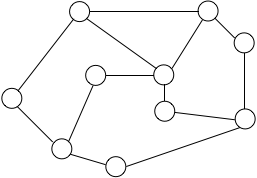
\includegraphics[scale=0.6]{FiguresGraph/EulerienInitial}
       \caption{Example of an instance of the chinese postman with $10$ cross vertices.}
              \label{fig:eulerianInitial}
\end{center}
\end{figure}

\bigskip

This problem may be formulated mathematically in term of eulerian cycles.
Intuitively, the basic idea is to duplicate some edges that are carefully chosen in order to use the previous construction
of an eulerian tour of section~\ref{sec:eulerianCycle} that will help the postman to determine 
the optimal tour (of minimal length) using some simple mathematical properties. 
\bigskip

First, we know that there is an even number of odd vertices.
Considering the previous instance of the postman problem, there are $4$ such vertices (represented in grey in Fig.~\ref{fig:eulerianVodd}).

\begin{figure}[h]
\begin{center}
       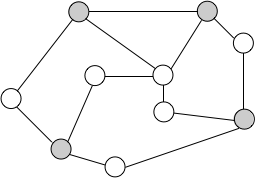
\includegraphics[scale=0.6]{FiguresGraph/EulerienVodd}
       \caption{The $4$ vertices with an odd degree in the previous instance.}
              \label{fig:eulerianVodd}
\end{center}
\end{figure}
\bigskip

As there exists a path between any pair of vertices of odd degree in $V_{odd}$,
we consider the complete graph whose vertices are the odd degree vertices weighting the edges with the shortest paths (denoted by $K_{odd}$).
As we mentioned in the preliminary properties, computing the shortest paths is a classical problem, which can be solved in polynomial time. 

\begin{figure}[h]
\begin{center}
       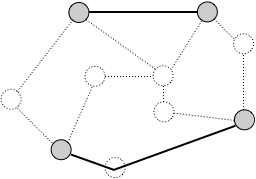
\includegraphics[scale=0.6]{FiguresGraph/EulerienPerfectMatching}
       \caption{The minimum weight perfect matching labelled by the shortest distances between the vertices of $V_{odd}$.}
              \label{fig:eulerianperfectmatching}
\end{center}
\end{figure}
\bigskip

Then, it is possible to do the correspondence between the optimal solution of the postman problem and a perfect matching of minimal weight in $K_{odd}$
%Recall that a matching is a set of edges without common vertices. It is perfect if it has the maximum number of edges. 
by duplicating the edges of the minimal perfect matching.

\begin{figure}[h]
\begin{center}
       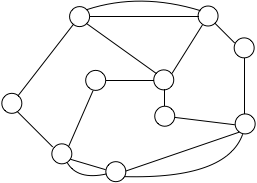
\includegraphics[scale=0.6]{FiguresGraph/EulerienFinal}
       \caption{Final step: adding the edges of the minimum perfect matching.}
              \label{fig:eulerianFinal}
\end{center}
\end{figure}

The main steps of the algorithm for determining the optimal tour are the following:

\begin{itemize}
\item Consider the complete graph with the odd vertices and compute its weight by the shortest paths.
Compute a perfect matching of minimal weight between these vertices. 
\item Duplicate all the edges along the paths of this matching.
\item Determine an eulerian tour in this new graph with even degrees.
\end{itemize}

The optimality of this algorithm comes from the fact that the duplicated edges are the minimum possible ones.
% This is straightforward for two odd vertices.
Finally, all the vertices of the new graph are even since the degree of the odd vertices in $G$ is augmented by $1$
(extremities of the paths) and the other even vertices which are intermediate vertices of the paths remain even. 


%%%%%%%%%%%%%%%%%%%%%%%%%%%%%%%%%%%%%%%%%

\section{Hamiltonian tours}

\cite{Fleischner74}
(square of 2-connected graph is hamiltonian)

Let us now turn to the problem of cycles going through the vertices of a given graph instead of edges.
\bigskip

\noindent {\bf Definition.}
An hamiltonian cycle is a tour that visits all vertices exactly once.

This problem is the traveling salesman problem, called TSP in short.
It corresponds to determine a minimal hamiltonian cycle in a weighted complete graphs $K_n$.
Obviously, $K_n$ is hamiltonian (it exists $n!$ such hamiltonian paths), thus, the question here is to determine the minimum one. 

TSP is a classical problem in Operational Research.
Let us consider a saleswoman who wants to organize the visit of her clients as best as possible.
It consists in visiting them in various cities with her vehicle. 
Of course, she must go in every city and her objective is to minimize the total distance done in the tour. 
The only information she has is the list of the cities and a map with all inter-cities distances. 
We assume a \textit{Euclidian distance} (for instance the weights correspond to number of kilometers between two cities).
This property means that the straight line is always the minimum distance, or in other words that the distance between two vertices/cities
is larger if the path is going through any other vertex. 
%More formally, the input of the problem is a weighted matrix with an infinite weight on the diagonal.
\bigskip

\noindent {\bf Proposition.}
The solution of Christofides algorithm is not worse than $\frac{3}{2}$ time the optimal tour.
\bigskip

Let us construct an efficient solution for this problem. It is well-known that TSP is a hard problem, 
that means we can not expect a polynomial time algorithm which solves exactly the problem, unless $\mathcal{P} = \mathcal{NP}$. 
Fig.~\ref{fig:perfectMatchingInitial} presents an example of euclidian TSP with $n=7$ cities. 
\begin{figure}[h]
\begin{center}
       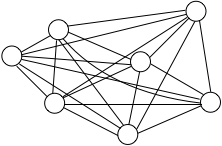
\includegraphics[scale=0.8]{FiguresGraph/christofides1}
       \caption{Example of an instance of TSP with 7 cities.}
              \label{fig:christofidesInitial}
\end{center}
\end{figure}

Let us construct a good solution (not \textit{too far} from the optimal) in polynomial time. 
Let us denote by $\omega_G$ the weight of graph G (i.e. the sum of the weights on its edges). 
The Chritofides algorithm proceeds in three steps. 
\bigskip

\textbf{Step 1.} Determine a minimal weight spanning tree $T^*$. 
%A spanning tree of G is a tree (connected graph with no cycle) with the same set of vertices as G. 
As we recalled in the preliminaries, a minimal weight spanning tree can be determined in polynomial time. 
\bigskip

$\omega_{T^*}$ is a lower bound of the value of the optimal tour $\omega_{H^*}$. 
Indeed, $H^*$ is a cycle, then, removing any edge in $H^*$ leads to a chain, which is a particular spanning tree.
As $T^*$ is the minimal spanning tree, we have:
$\omega_{T^*} \leq \omega_{H^*}$.

\begin{figure}[h]
\begin{center}
       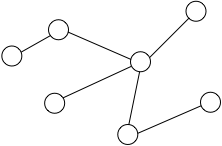
\includegraphics[scale=0.6]{FiguresGraph/christofides2}
       \caption{Construction of an optimal spanning Tree $T^*$.}
              \label{fig:christofidesSpanningTree}
\end{center}
\end{figure}


\textbf{Step 2.} Consider now the set $V_{odd}$ of the vertices of $T^*$ whose degrees are odd. 

We proved in the preliminary properties that the cardinality of $V_{odd}$ is even. 

Let us construct the perfect matching $C^*$ of minimum weight between the vertices in $V_{odd}$. 
Fig.~\ref{fig:AllPerfectMatchings} shows all possible perfect matchings on the previous example, the optimal one (with minimal weight) is represented in bold. 
\begin{figure}[h]
\begin{center}
       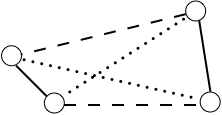
\includegraphics[scale=0.6]{FiguresGraph/perfectmatchingAll}
       \caption{The three different perfect matchings on the set of four vertices of odd degree.
       The optimal one is represented in bold (the two others are in dashed and dot lines).}
              \label{fig:AllPerfectMatchings}
\end{center}
\end{figure}

Fig.~\ref{fig:christofidesPerfectMatching} illustrates the graph obtained by considering the edges of both $T^*$ and $C^*$. 
\begin{figure}[h]
\begin{center}
       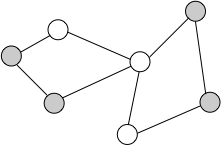
\includegraphics[scale=0.6]{FiguresGraph/christofides3}
       \caption{Adding the optimal perfect matching $C^*$ to the minimal spanning tree $T^*$.}
              \label{fig:christofidesPerfectMatching}
\end{center}
\end{figure}

Let us now determine a lower bound of the optimal tour $H^*$ (represented in Fig.~\ref{fig:perfectMatchingInitial}).

$2 \omega_{C^*}$ is a lower bound of the value of the optimal tour ($\omega_{C^*} \leq \frac{1}{2} \omega_{H^*}$). 
Indeed, consider first the perfect matching $C^*$.
As its vertices belong to $H^*$, $\omega_{C*}$ is lower than the piece of hamiltonian tour contained between these vertices
because of the euclidian property (see Fig.~\ref{fig:perfectMatchingC*}).
Similarly for the \textit{complementary} perfect matching $C$ (Fig.~\ref{fig:perfectMatchingC}).  
Thus, the weight of the cycle formed by the concatenation of both perfect matchings is lower than the hamiltonian tour $\omega_{C^* \bigcup C} \leq \omega_{H^*}$.
Moreover, as $C^*$ is the minimum perfect matching, we have $\omega_{C^*} \leq \omega_{C}$, this concludes the proof.


\begin{figure}[h]
\begin{center}
       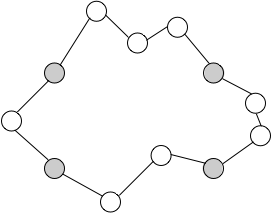
\includegraphics[scale=0.7]{FiguresGraph/perfectmatching1}
       \caption{An optimal hamiltonian cycle $H^*$.}
              \label{fig:perfectMatchingInitial}
\end{center}
\end{figure}

\begin{figure}[h]
\begin{center}
       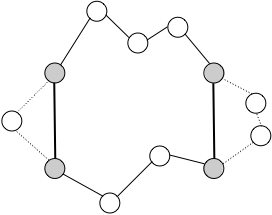
\includegraphics[scale=0.7]{FiguresGraph/perfectmatching2}
       \caption{Perfect matching $C^*$ between the vertices of odd degrees.}
              \label{fig:perfectMatchingC*}
\end{center}
\end{figure}

\begin{figure}[h]
\begin{center}
       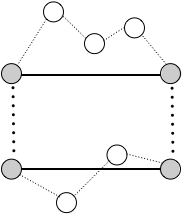
\includegraphics[scale=0.7]{FiguresGraph/perfectmatching3}
       \caption{Cycle $C^* \bigcup C$ (in dashed and bold).}
              \label{fig:perfectMatchingC}
\end{center}
\end{figure}

\bigskip

\textbf{Step 3.} 
All the vertices of $T^* \cup C^*$ have an even degree since we added an edge of $C^*$ to every odd degree vertices of $T^*$. 
We are now going to transform this graph by replacing iteratively the high degree vertices by shortcuts, which decreases the degree until reaching $2$. 

While it exists a vertex of degree greater than 4, we remove two of these consecutive edges and replace them by the opposite edge of this triangle 
without disconnecting the graph. There are $2k$ ways to remove $2$ edges and replace them by the triangle edge. Some of them disconnect the graph
and thus, must be avoided. 
Fig.~\ref{fig:christofidesFinalStep1} shows such a transformation on the previous example, 
Fig.~\ref{fig:christofidesFinalStep2} shows a valid transformation.

\begin{figure}[h]
\begin{center}
       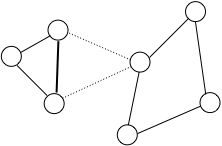
\includegraphics[scale=0.6]{FiguresGraph/christofides4}
       \caption{Reduction of the degree in $T^* \bigcup C^*$, disconnected solution.}
              \label{fig:christofidesFinalStep1}
\end{center}
\end{figure}

\begin{figure}[h]
\begin{center}
       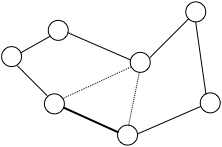
\includegraphics[scale=0.6]{FiguresGraph/christofides5}
       \caption{Reduction of the degree in $T^* \bigcup C^*$, connected solution.}
       \label{fig:christofidesFinalStep2}
\end{center}
\end{figure}

This process leads to a feasible tour. 
Such transformations do not increase the total weight.

Finally, 
as $\omega_{T^*} \leq \omega_{H^*}$ and $\omega_{C^*} \leq 1/2 \omega_{H^*}$,
we deduce that the value of such a tour is lower than $3/2 \omega_{H^*}$.
 


\section{Hypergraphs: an advanced topic}

When studying certain computing-related topics, one will
need a generalization of graphs called {\em hypergraphs}.  A
hypergraph has nodes that are analogous to the nodes of a graph, but
in place of edges a hypergraph has {\em hyperedges}.  Each hyperedge
is a set of nodes whose size is not restricted to $2$; thus,
hypergraphs represent internode relationships that are not ``binary''.
A simple example can be framed by describing {\em bus-connected}
systems, such as occur in certain genres of digital circuits and
certain message-passing systems.  The underlying idea is that nodes
that coreside in a hyperedge represent agents that ``hear'' all
messages simultaneously, or equi-potential points in a network.
Because of their inherent complexity, hypergraphs as graph-theoretic
objects are usually relegated to advanced courses, but specific
concrete instantiations, exemplified by bus-oriented communication and
digital circuits should be accessible even to early students.


